\documentclass[a4paper, 12pt]{article}

\usepackage{cmap}
\usepackage{mathtext} 
\usepackage[T2A]{fontenc}
\usepackage[utf8]{inputenc}
\usepackage[english,russian]{babel}	

\usepackage{amsfonts,amssymb,amsthm,mathtools}
\usepackage{amsmath}
\usepackage{icomma} 

\usepackage{graphicx} 
\graphicspath{{Picturies/}, {Theory/}}
\usepackage{wrapfig}

\usepackage{array,tabularx,tabulary,booktabs}
\usepackage{longtable}
\usepackage{multirow}

\usepackage{caption}
\captionsetup{labelsep=period}

\renewcommand{\phi}{\varphi}
\newcommand{\eps}{\varepsilon}
\newcommand{\parag}[1]{\paragraph*{#1:}}

\newcounter{Points}
\setcounter{Points}{1}
\newcommand{\point}{\arabic{Points}. \addtocounter{Points}{1}}

\author{Вязовцев Андрей, Б01-005}
\date{24.03.21}
\title{Лабораторная работа 2.2.1. Исследование взаимной диффузии газов.}

\begin{document}

\maketitle

\newpage

\parag {Цель работы}
1) регистрация зависимости концентрации гелия в воздухе от времени с помощью датчиков теплопроводности при начальных давлениях смеси газов; 2) определение коэффициента диффузии по результатам измерений.

\parag {В работе используются}
измерительная установка; форвакуумный насос; баллон с газом (гелий); манометр; источник питания; магазин сопротивлений; гальзанометр; секундомер.

% Я бы мог нормально написать теорию, но... Зачем? Мой одногруппник отправил 
% ей лабу, в которой был титульнык, 7 страниц таких скринов, а ход работы
% напечатан 228-ым шрифтом с огромной табличкой и картинками.
% И зачем после этого стараться? Зачем? Чтобы в очередной раз получить
% унижение от неё на сдаче? Нет, спасибо. Иди нахуй.
% Когда-нибудь все люди станут адекватными.
% Когда-нибудь.

\includegraphics[height = 470px, width = \textwidth]{"1.png"}
\newpage
\includegraphics[scale = 1.2]{"2.png"}
\newpage
\includegraphics[scale = 1.2]{"3.png"}
\newpage
\includegraphics[scale = 1.2]{"4.png"}
\newpage
\includegraphics[scale = 1.2]{"5.png"}

\parag{Экспериментальная установка} ~\\ \\ \\
\includegraphics[scale = 1]{"Workplace.png"}

Особенности установки:

Кран $К_4$ обладает повышенной вакуумплотностью и используется для изолирования измерительной части установки от возможных протечек гелия и воздуха. Двухходовой кран $К_5$ служит для подключения форвакуумного насоса к установке, подачи воздуха в установку и соединения форвакуумного насоса с атмосферой. Устройство и назначение кранов $К_6$ и $К_7$ подачи гелия соответствуют основному описанию.
\newpage

\parag {Ход работы} ~\\

\point Подготовим установку к работе. Ознакомимся с расположением кранов у неё.

\point Измерим показания вольтметра во время диффузии. Для этого будем настраивать вольтметр под рабочее давление $p_{\text{раб}}$, а после будем запускать в верхний сосуд водород с давлением $p_{H_2} = 0,2 p_{\text{раб}}$, в нижний --- воздух с $p_{\text{возд}} = 1,75 p_{\text{раб}}$, затем начинать процесс и ждать снижения показаний вольтметра на $30-50\%$. Повторим данные действия при нескольких рабочих давлениях: 1) 40 тор, 2) 100 тор, 3) 150 тор, 4) 200 тор, 5) 300 тор. Данные внесём в таблицу:

\begin{longtable}{|c|c|c|c|c|c|}
    \hline
    t, с & $U_1$, мВ & $U_2$, мВ & $U_3$, мВ & $U_4$, мВ & $U_5$, мВ \\ \hline
    \endfirsthead
    \hline
    t, с & $U_1$, мВ & $U_2$, мВ & $U_3$, мВ & $U_4$, мВ & $U_5$, мВ \\ \hline
    \endhead
    \hline
    \endfoot
    \hline
    \endlastfoot 
    0	& 19.96	& 20.43 & 23.74 & 27.81 & 26.34 \\
    10	& 19.35	& 20.13 & 23.45 & 27.65 & 26.13 \\
    20	& 18.81	& 19.85 & 23.22 & 27.49 & 25.95 \\
    30	& 18.27	& 19.56 & 22.99 & 27.36 & 25.73 \\
    40	& 18.06	& 19.18 & 22.78 & 27.22 & 25.52 \\
    50	& 17.25	& 19.01 & 22.55 & 27.07 & 25.32 \\
    60	& 16.74	& 18.75 & 22.33 & 26.95 & 25.12 \\
    70	& 16.29	& 18.49 & 22.13 & 26.81 & 24.92 \\
    80	& 15.84	& 18.25 & 21.92 & 26.68 & 24.73 \\
    90	& 15.41	& 18.01 & 21.73 & 26.55 & 24.59 \\
    100	& 14.98	& 17.78 & 21.55 & 26.42 & 24.36 \\
    110	& 14.56	& 17.54 & 21.37 & 26.31 & 24.18 \\
    120	& 14.17	& 17.32 & 21.18 & 26.16 & 24.01 \\
    130	& 13.79	& 17.11 & 21.01 & 26.04 & 23.83 \\
    140	& 13.39	& 16.88 & 20.83 & 25.92 & 23.66 \\
    150	& 13.03	& 16.68 & 20.67 & 25.79 & 23.49 \\
    160	& 12.66	& 16.47 & 20.49 & 25.66 & 23.31 \\
    170	& 12.34	& 16.25 & 20.32 & 25.54 & 23.14 \\
    180	& 12.02	& 16.07 & 20.15 & 25.42 & 22.98 \\
    190	&    ~  & 15.88 & 19.98 & 25.31 & 22.83 \\
    200	&    ~  & 15.69 & 19.83 & 25.17 & 22.67 \\
    210	&    ~  & 15.49 & 19.66 & 25.05 & 22.51 \\
    220	&    ~  & 15.31 & 19.57 & 24.94 & 22.37 \\
    230	&    ~  & 15.12 & 19.34 & 24.82 & 22.21 \\
    240	&    ~  & 14.95 & 19.18 & 24.72 & 22.06 \\
    250	&    ~  & 14.76 & 19.02 & 24.61 & 21.91 \\
    260	&    ~  & 14.58 & 18.87 & 24.48 & 21.76 \\
    270	&    ~  & 14.41 & 18.73 & 24.37 & 21.62 \\
    280	&    ~  & 14.23 & 18.57 & 24.26 & 21.47 \\
    290	&    ~  & 14.06 & 18.42 & 24.16 & 21.33 \\
    300	&    ~  & 13.89 & 18.27 & 24.05 & 21.19 \\
    310	&    ~  & 13.73 & 18.13 & 23.94 & 21.04 \\
    320	&    ~  & 13.57 & 17.98 & 23.83 & 20.91 \\
    330	&    ~  & 13.41 & 17.83 & 23.73 & 20.76 \\
    340	&    ~  & 13.08 & 17.71 & 23.61 & 20.63 \\
    350	&    ~  & 12.93 & 17.43 & 23.51 & 20.49 \\
    360	&    ~  & 12.78 & 17.29 & 23.41 & 20.35 \\
    370	&    ~  & 12.63 & 17.15 & 23.31 & 20.22 \\
    380	&    ~  & 12.48 & 17.02 & 23.19 & 20.09 \\
    390	&    ~  & 12.33 & 16.88 & 23.08 & 19.95 \\
    400	&    ~  & 12.19 & 16.75 & 22.97 & 19.83 \\
    410	&    ~  & 12.06 & 16.62 & 22.87 & 19.71 
\end{longtable}

\point Построим графики $U(t)$ и $\ln U(t)$.

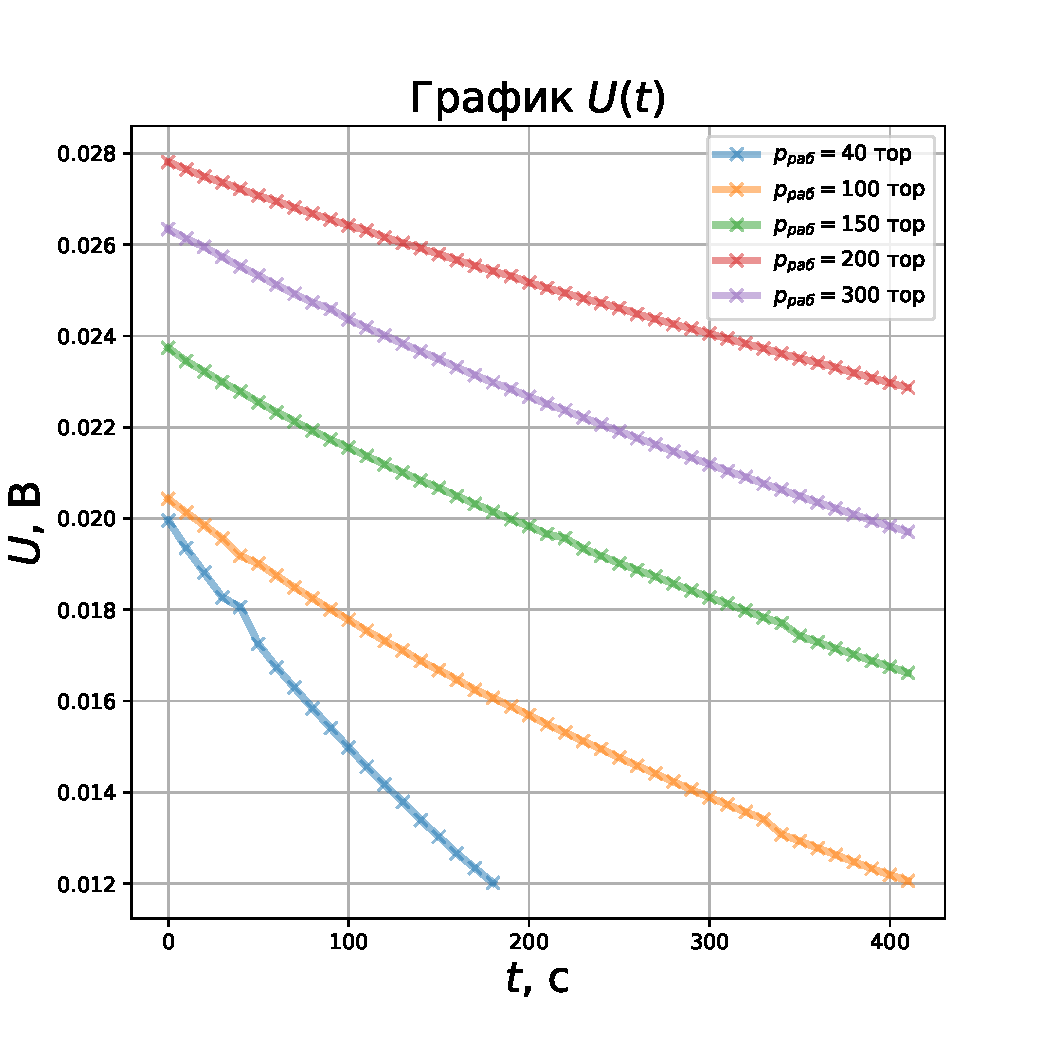
\includegraphics[scale = 0.6]{Picturies/exp.pdf} \\
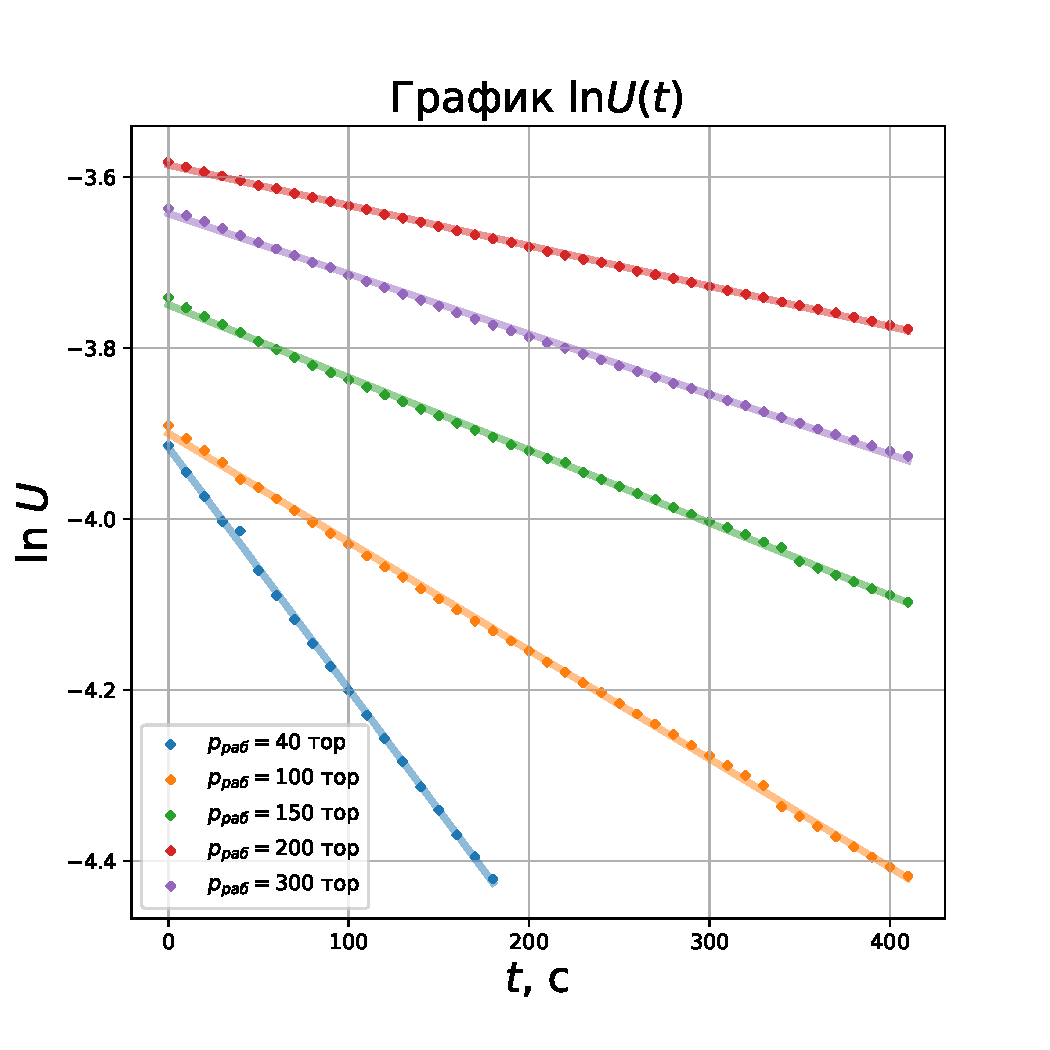
\includegraphics[scale = 0.6]{Picturies/ln.pdf}

\point Найдём для каждого графика коэффициент диффузии по формуле:

\[
    D = - \frac {kVL}{2S}
\]

Для этого воспользуемся следующими параметрами установки: $V = 1200 \pm  30 ~ \text{см}^3$, $\displaystyle \frac{L}{S} = 5,5 \pm 0,5 ~ \frac{1}{\text{см}}$ Так же посчитаем погрешности их вычисления.

\begin{align*}
    D_1 &= 9,3 \pm 1,0 ~ \frac{\text{см}^2}{\text{с}} & \eps_1 &= 11\% \\
    D_2 &= 4,2 \pm 0,4 ~ \frac{\text{см}^2}{\text{с}} & \eps_2 &= 10\% \\
    D_3 &= 2,8 \pm 0,3 ~ \frac{\text{см}^2}{\text{с}} & \eps_3 &= 10\% \\
    D_4 &= 1,6 \pm 0,2 ~ \frac{\text{см}^2}{\text{с}} & \eps_4 &= 10\% \\
    D_5 &= 2,3 \pm 0,3 ~ \frac{\text{см}^2}{\text{с}} & \eps_5 &= 11\% 
\end{align*}

\point Теперь построим график $\displaystyle D (\frac{1}{T})$. 

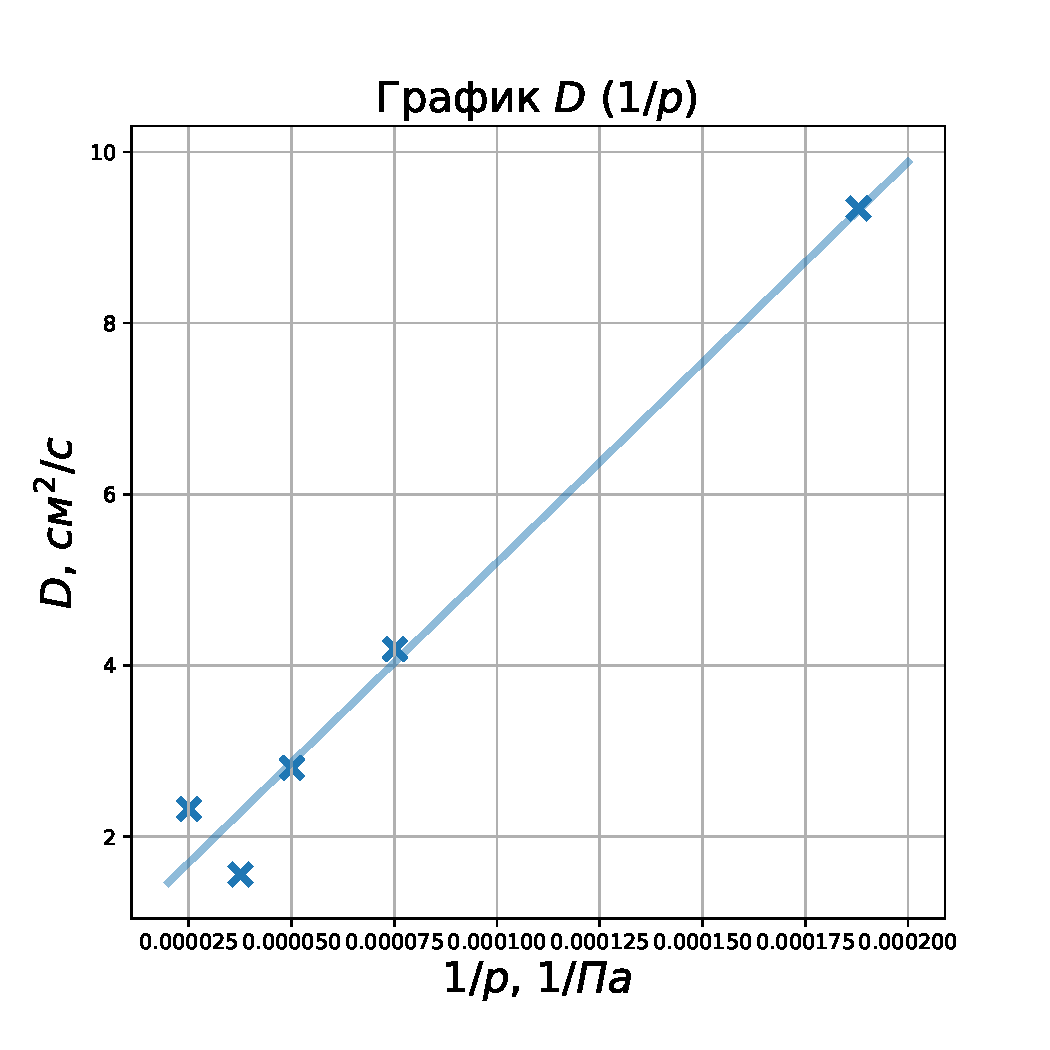
\includegraphics[scale = 0.6]{Picturies/inv.pdf}

\point Оценим длину свободного пробега атомов гелия в воздухе $\lambda_{\text{He}}$:

\[
    \lambda_{\text{He}} = \frac{3D}{\langle v \rangle} = 3D \sqrt{\frac{\pi \mu}{8RT}} \approx 180 \pm 20 \text{ нм}
\]

Оценим эффективное сечение столкновений $\sigma_{\text{He - возд}}$ при атмосферном давлении:

\[
    \sigma_{\text{He - возд}} = \frac{1}{\lambda n} = \frac{kT}{\lambda P} \approx (2,2 \pm 0,2) \cdot 10^{-19} \text{ м}
\]

\parag{Вывод} ~\\

Если экстраполировать график функции $\displaystyle D ~(\frac{1}{p})$, то можно получить примерное значение коэффициента диффузии при $P = 1$ атм, оно равно $D \approx 0,99 ~ \frac{\text{см}^2}{\text{с}}$. Табличное значение же составляет $D = 0,62 ~ \frac{\text{см}^2}{\text{с}}$. Таким образом, отклонение от реального значения составило 60\%. Если учесть, что эти коэффициенты вычислены для различных температур, то сравнивать эти значения не совсем корректно, и оценить точность методики сложно.

Но зато значение длины пробега $\lambda_{\text{He}}$ совпало с табличным. Это может свидетельствовать о корректности нашего способа измерения.

\end{document}

